\documentclass[11pt,letterpaper]{article}
\usepackage[utf8]{inputenc}
\usepackage{amsmath}
\usepackage{amsfonts}
\usepackage{amssymb}
\usepackage[utf8]{inputenc}
\usepackage{listings}
\usepackage{float}
\usepackage[margin=1in]{geometry}
\setlength\parindent{0pt}
\usepackage{xcolor}
\usepackage{graphicx}
\definecolor{dkgreen}{rgb}{0,0.6,0}
\definecolor{dred}{rgb}{0.545,0,0}
\definecolor{dblue}{rgb}{0,0,0.545}
\definecolor{lgrey}{rgb}{0.9,0.9,0.9}
\definecolor{gray}{rgb}{0.4,0.4,0.4}
\definecolor{darkblue}{rgb}{0.0,0.0,0.6}
\lstdefinelanguage{python}{
      backgroundcolor=\color{lgrey},  
      basicstyle=\footnotesize \ttfamily \color{black} \bfseries,   
      breakatwhitespace=false,       
      breaklines=true,               
      captionpos=b,                   
      commentstyle=\color{dkgreen},   
      deletekeywords={...},          
      escapeinside={\%*}{*)},                  
      frame=single,                  
      language=C++,                
      keywordstyle=\color{purple},  
      morekeywords={BRIEFDescriptorConfig,string,TiXmlNode,DetectorDescriptorConfigContainer,istringstream,cerr,exit}, 
      identifierstyle=\color{black},
      stringstyle=\color{blue},      
      numbers=right,                 
      numbersep=5pt,                  
      numberstyle=\tiny\color{black}, 
      rulecolor=\color{black},        
      showspaces=false,               
      showstringspaces=false,        
      showtabs=false,                
      stepnumber=1,                   
      tabsize=5,                     
      title=\lstname,                 
    }
\author{Paul Ely, Jason Dorweiler, Kabir Kang}
\title{Project 3 - Linear Programming}
\begin{document}

\maketitle

\section*{Problem 1: mmmmm ... pork}

\paragraph{Objective.} We want to maximize the profits of a factory that produces hams, pork bellies, and picnic hams. Each of these products can be sold fresh or smoked. To solve this problem, consider the following variables: \\

\begin{tabular}{ll}
Variable & Definition \\
\hline
$H_F$ & Fresh hams \\
$H_R$ & Hams smoked on regular time \\
$H_O$ & Hams smoked on overtime \\
$B_F$ & Fresh pork bellies \\
$B_R$ & Pork bellies smoked on regular time \\
$B_O$ & Pork bellies smoked on overtime \\
$P_F$ & Fresh picnic hams \\
$P_R$ & Picnic hams smoked on regular time \\
$P_O$ & Picnic hams smoked on overtime \\
\end{tabular}

Our objective is to maximize the net profit (N) equation given by:
$N = 8 H_F + 14 H_R + 11 H_O + 4 B_F + 12 B_R + 7 B_R + 4 P_F + 13 P_R + 9 P_O$

\paragraph{Constraints.} The production of hams is subject to the following constraints:

\begin{itemize}
\item[] \textit{There are 480 hams, 400 pork bellies, and 230 picnic hams produced daily}. $H = 480$, $B = 400$, $P = 230$
\item[] \textit{Only 420 items can be smoked in regular time per day}. $H_R + B_R + P_R <= 420$
\item[] \textit{Only 250 items can be smoked in overtime.} $H_O + B_O + P_O <= 250$
\end{itemize}

\paragraph{Linear equation.} The linear equation matrix is as follows: \\
\begin{align*}
max: 8 H_F &+ 14 H_R + 11 H_O \\
+ 4 B_F &+ 12 B_R + 7 B_R \\ 
+ 4 P_F &+ 13 P_R + 9 P_O
\end{align*}
\begin{align*}
s.t.: H_F + H_R + H_O &= 480 \\
B_F + B_R + B_O &= 400 \\
P_F + P_R + P_O &= 230 \\
H_R + B_R + P_R &<= 420 \\
H_O + B_O + P_O &<= 250
\end{align*}

\paragraph{Optimal solution.} We found the optimal solution to be: \\
\begin{tabular}{|c|c|c|c|}
\hline 
& Fresh & Smoked (regular time) & Smoked (overtime) \\ 
\hline 
Hams & 440 & 0 & 40 \\ 
Pork belly & 0 & 400 & 0 \\ 
Picnic ham & 0 & 20 & 210 \\ 
\hline 
\multicolumn{3}{|c}{Total Net Profit:} & $\$$10910.00 \\ 
\hline 
\end{tabular} 

\paragraph{Language/solver environment.} We used Python with the PuLP math package to solve the optimization problem.

Each of the variables are declared using LpVariable().  There are additional options to add a printable variable name and minimum/maximum constraints, in this case 0.

The problem is set up using LpProblem().  In here we specify that we want to maximize our objective with LpMaximize.

Next we set up the objective to maximize on line 18. This is the same objective that we defined at the beginning of this report. 

Starting on line 21 we enter in each of the constraints for the problem and then just run prob.solve(). Note: that we left out parts of the program to display results since it is not relevant for this report.  

\begin{lstlisting}[language=python,caption={Code to solve linear program},mathescape]
//set up variables, minimum of 0 for each
HAM_FRESH = LpVariable("ham fresh", 0)
HAM_SRT = LpVariable("Ham Smoked RT", 0)
HAM_SOT = LpVariable("Ham Smoked OT", 0)

PORK_FRESH = LpVariable("PORK fresh", 0)
PORK_SRT = LpVariable("PORK Smoked RT", 0)
PORK_SOT = LpVariable("PORK Smoked OT", 0)

P_HAM_FRESH = LpVariable("P-ham fresh", 0)
P_HAM_SRT = LpVariable("P-Ham Smoked RT", 0)
P_HAM_SOT = LpVariable("P-Ham Smoked OT", 0)

// Create the 'prob' variable to contain the problem data
prob = LpProblem("Pork Profit", LpMaximize)

// objective to solve
prob += HAM_FRESH*8+HAM_SRT*14+HAM_SOT*11+PORK_FRESH*4+PORK_SRT*12+PORK_SOT*7+P_HAM_FRESH*4+P_HAM_SRT*13+P_HAM_SOT*9

// constraints
prob += HAM_FRESH+HAM_SRT+HAM_SOT <=480 // at most 480 ham
prob += PORK_FRESH+PORK_SRT+PORK_SOT <= 400 // at most 400 pork
prob += P_HAM_FRESH+P_HAM_SRT+P_HAM_SOT <= 230 // at most 230 picnic ham
prob += HAM_SRT+PORK_SRT+P_HAM_SRT <= 420 // max 420 smoked on RT
prob += HAM_SOT+PORK_SOT+P_HAM_SOT <= 250 // max 250 smoked on OT

// The problem data is written to an .lp file
prob.writeLP("porkprofit.lp")

// The problem is solved using PuLP's choice of Solver
prob.solve()

\end{lstlisting}


\section*{Problem 2: }

\paragraph{Objective.} \bigskip The objective here is to minimize the maximum absolute error between each point in the given data set and a regression line. Since the absolute value is not a linear function we have to split the equation into two.  

Let E be the error and c be some constant. Then this equation is: 

\begin{align*}
 min: \bigskip &|ax + by +c| \\
 Constraints: \bigskip E &>= y_i - (x_i * x + c) \\
 E &>= -y_i + (x_i * x + c)
\end{align*}


\paragraph{Best Solution.} \bigskip We found the optimal solution as follows:

\begin{align*}
 E &= 0.571429 \\
 x &= 1.71429 \\
 C &= 1.85714 
\end{align*}

The setup for this problem is very similar to problem one.   We set our variables x,y,c as global to use them for our plotting function (not shown).  The points are stored in the points array.  A constraint is added for each individual point using both of the constraint equations defined above.  This time we set it up to minimize the objective (error) by using LpMinimize. 

\begin{figure}[h!]
\centering
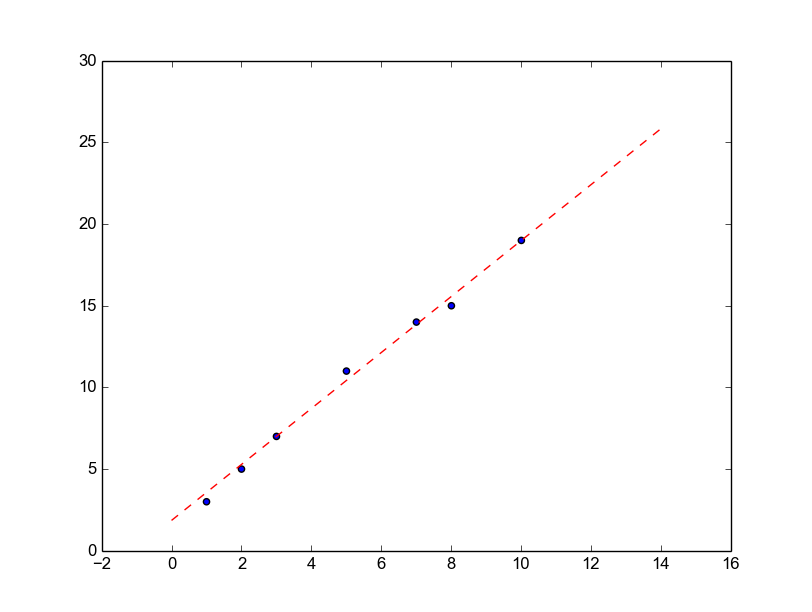
\includegraphics[width=0.8\textwidth]{figure_1}
\caption{Plot of the best solution}
\end{figure} 

\pagebreak 

\begin{lstlisting}[language=python,caption={Code to solve linear program},mathescape]

//set up variables
x = LpVariable("X_i")
y = LpVariable("Y_i")
c = LpVariable("C")
error = LpVariable("Error")


def main():

	global x, y, c

	points = [[1,3], [2,5], [3,7], [5,11], [7,14], [8,15], [10,19]]

	// Create the 'prob' variable to conmitain the problem data
	prob = LpProblem("min max line", LpMinimize)

	// objective to minimize
	prob += error

	// add constraints
	for i in range(len(points)):
		prob += error >= points[i][1] - (points[i][0] * x +c)
		prob += error >= -points[i][1] + (points[i][0] * x +c)
	
	// The problem data is written to an .lp file
	prob.writeLP("minmaxline.lp")

	// The problem is solved using PuLP's choice of Solver
	prob.solve()
	

\end{lstlisting}

\end{document}